\section{Software Development Life Cycle}
\emph{Software development life cycle} (SDLC) adalah proses terstruktur yang digunakan untuk merencanakan, membuat, menguji, dan menerapkan aplikasi perangkat lunak. SDLC berfungsi sebagai kerangka kerja yang menguraikan berbagai tahap yang terlibat dalam pengembangan perangkat lunak, memastikan bahwa perangkat lunak berkualitas tinggi disampaikan dengan efisien dan efektif. SDLC biasanya terdiri dari beberapa fase, termasuk analisis kebutuhan, desain, pengembangan, pengujian, penerapan, dan pemeliharaan \citep{chan2020devops}.
\singlespacing{}
Pada fase analisis kebutuhan, pemangku kepentingan mengumpulkan dan menganalisis kebutuhan serta harapan pengguna untuk mendefinisikan fungsionalitas perangkat lunak. Setelah itu, fase desain dilanjutkan, di mana arsitektur dan antarmuka pengguna perangkat lunak direncanakan. Fase pengembangan melibatkan pengkodean perangkat lunak yang sebenarnya, sementara fase pengujian memastikan bahwa perangkat lunak bebas dari cacat dan memenuhi persyaratan yang ditentukan. Setelah pengujian selesai, perangkat lunak diterapkan ke lingkungan produksi, dan pemeliharaan yang berkelanjutan dilakukan untuk menangani masalah yang muncul setelah penerapan \citep{chan2020devops}.
\singlespacing{}
SDLC sangat penting untuk mengelola kompleksitas pengembangan perangkat lunak, karena ia menyediakan peta jalan yang jelas bagi tim untuk diikuti, memfasilitasi manajemen proyek yang lebih baik dan komunikasi di antara pemangku kepentingan \citep{chan2020devops}.

\subsection{Model iteratif}

Model iteratif adalah salah satu model SDLC yang mengombinasikan proses-proses pada model waterfall dan model prototype. Model inkremental akan menghasilkan versi-versi perangkat lunak yang sudah mengalami penambahan fungsi.

\begin{figure}[htbp]
  \centering
  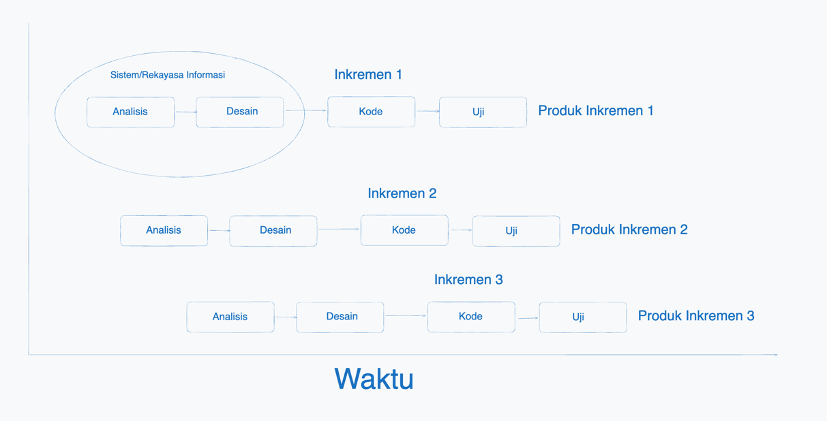
\includegraphics[width=0.85\linewidth]{images/bab-2/sdlc-iterative.png}
  \caption{Ilustrasi Model Iteratif}\label{fig:iterative-model}\citep{sukamto}
\end{figure}
